\section{Method}

\begin{figure*}
    \centering
    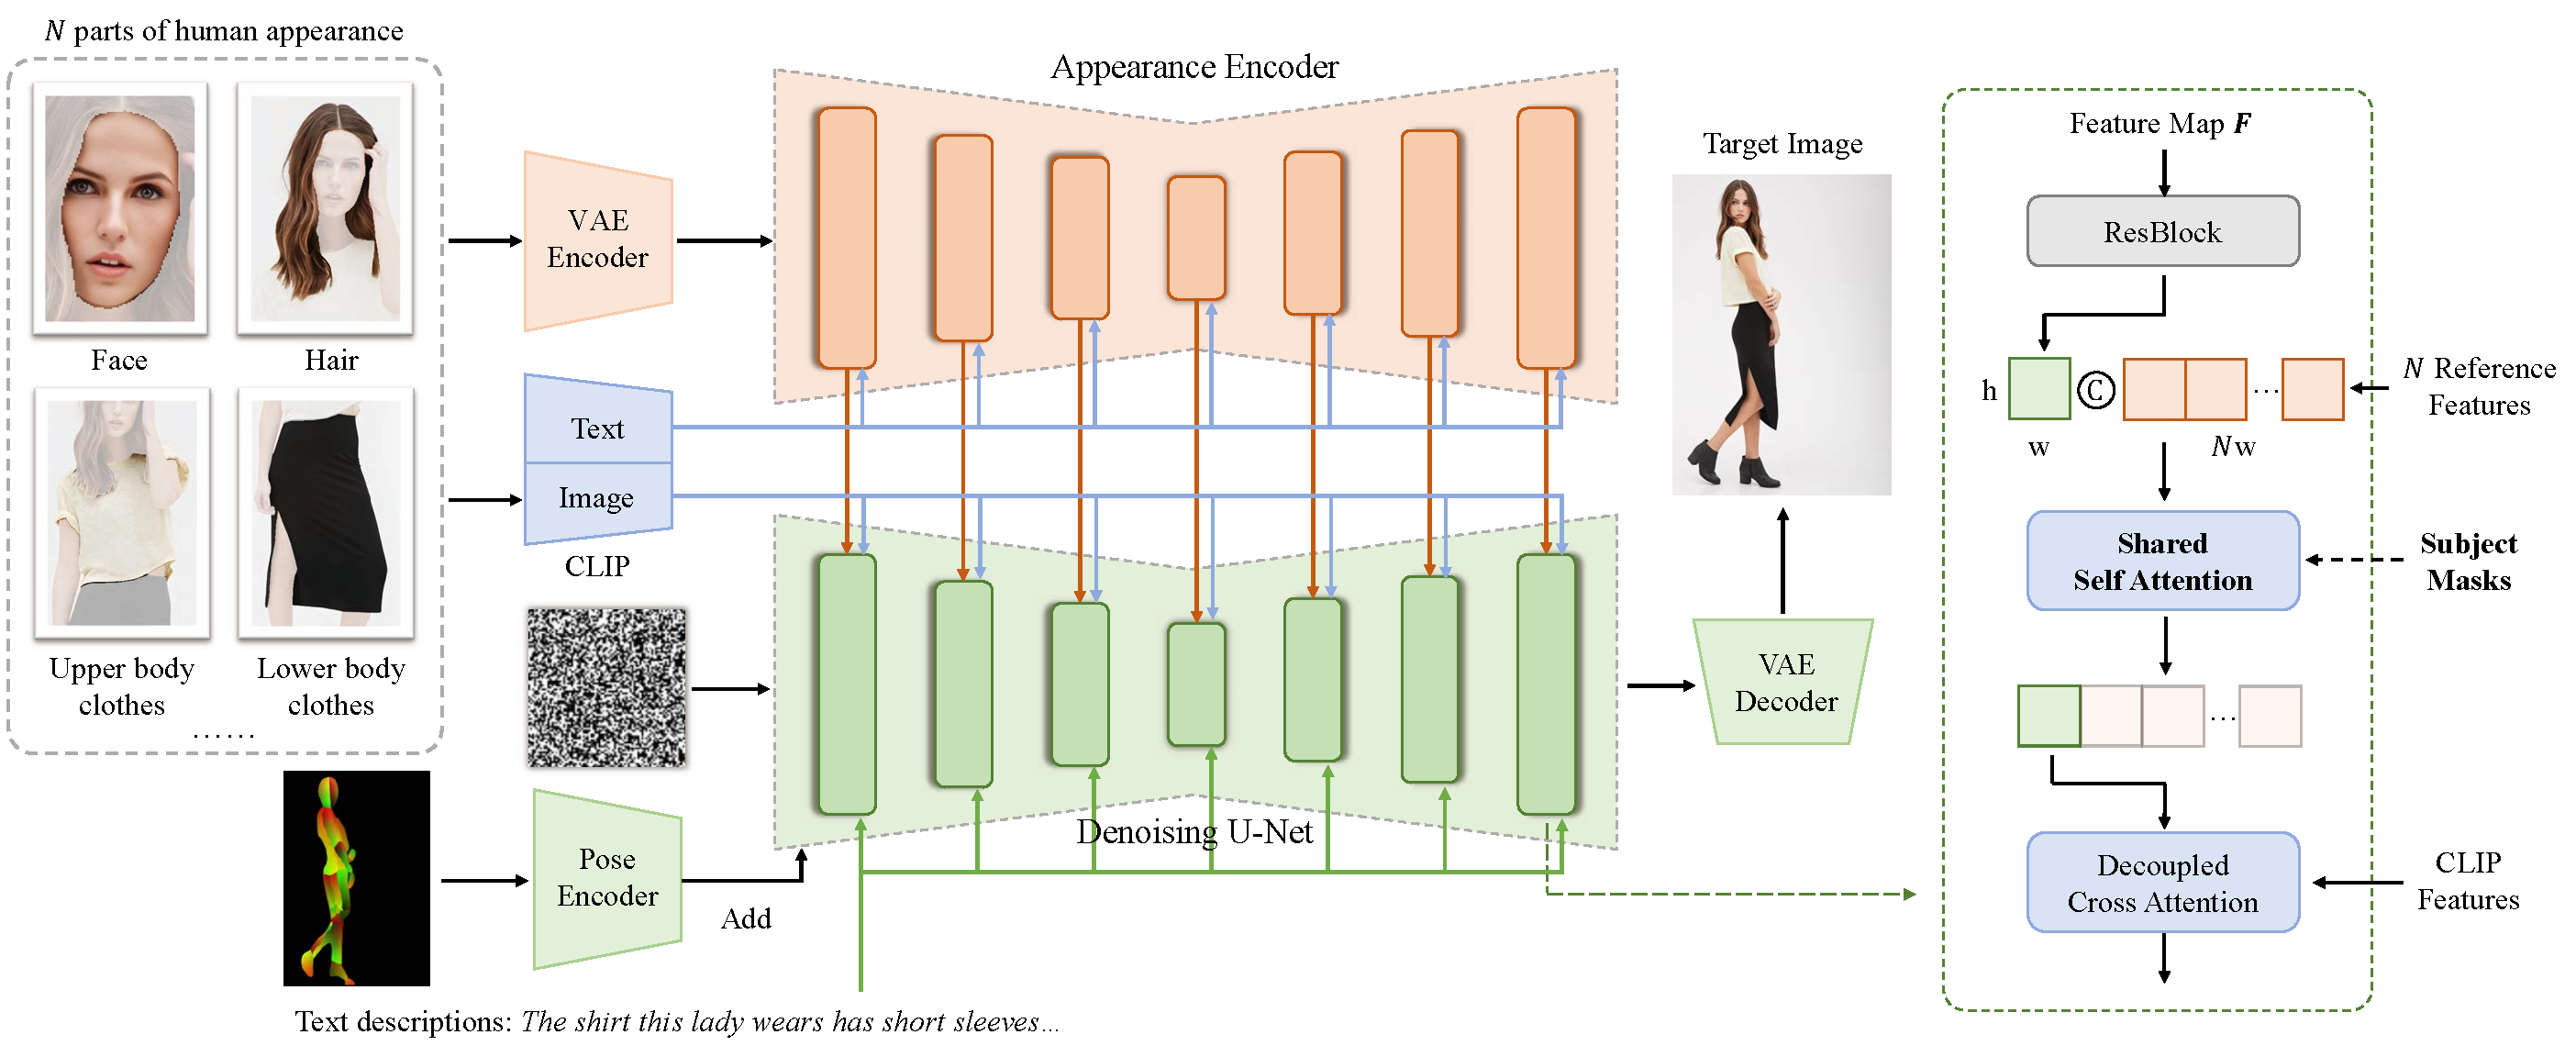
\includegraphics[width=\textwidth]{figure/overview.pdf}
    \caption{Overview of Parts2Whole. Based on the text-to-image diffusion model, our method designs an appearance encoder for encoding various parts of human appearance into multi-scale feature maps. We build this encoder by copying the network structure and pre-trained weights from denoising U-Net. Features obtained from reference images with their textual labels are injected into the generation process by shared attention mechanism layer by layer. To precisely select the specified parts from reference images, we enhance the vanilla self-attention mechanism by incorporating subject masks in the reference images. An illustration of one block in U-Net is shown on the right part.}
    \label{fig:overview}
\end{figure*}

We target controllable human image generation guided by multiple reference images. Given $N$ images that capture distinct parts of human appearance $\bm{x}^{1:N}$ and a pose map $\bm{p}$, and optionally text inputs, our objective is to synthesize a human image $\hat{\bm{x}}$ aligning with the specified appearances and posture. To achieve this goal, we propose Parts2Whole, a specialized framework designed to interpolate various reference images and generate high-quality portraits.

In general, Parts2Whole is built on text-to-image diffusion models~\cite{rombach2022ldm}. In the following sections, we start with an overview of T2I diffusion models, and in particular, the self-attention mechanism in Sec.~\ref{subsec:preliminaries}. We continue by presenting our unified reference framework in Sec.~\ref{subsec:unifiedref}, which consists of a semantic-aware appearance encoder, a shared self-attention that queries referential features within the self–attention layers, and the enhanced mask-guided subject selection. These methods enable Parts2Whole to accurately obtain the specific subject information from multiple reference images while preserving appearance details.

\subsection{Preliminaries}
\label{subsec:preliminaries}

\cparagraph{Text-to-Image Diffusion Models.}
Diffusion models~\cite{ho2020ddpm} exhibit promising capabilities in image generation. In this study, we select the widely adopted Stable Diffusion~\cite{rombach2022ldm} as our foundational model, which is also known as Latent Diffusion Models (LDM). The model operates the denoising process in the latent space of an autoencoder~\cite{kingma2022ae}, namely $\mathcal{E}(\cdot)$ and $\mathcal{D}(\cdot)$. During the training phase, an input image $\bm{x}_{0}$ is initially mapped to the latent space using a frozen encoder, yielding $\bm{z}_{0}=\mathcal{E}(\bm{x}_{0})$, then perturbed by a pre-defined Markov process:
\begin{equation}
    q(\bm{z}_{t}|\bm{z}_{t-1})=\mathcal{N}(\bm{z}_{t}; \sqrt{1-\beta_{t}}\bm{z}_{t-1}, \beta_{t}\bm{I})
    \label{eq:img_diff}
\end{equation}
For $t=1,\cdots, T$, where $T$ represents the number of steps in the forward diffusion process. The sequence of hyperparameters $\beta_{t}$ determines the noise strength at each step. The denoising UNet $\epsilon_{\theta}$ is trained to approximate the reverse process $q(\bm{z}_{t-1}|\bm{z}_{t})$. The training objective is expressed as:
\begin{equation}
    \mathcal{L}=\mathbb{E}_{\mathcal{E}(\bm{x}_{0}),\bm{\epsilon}\sim\mathcal{N}(\bm{0}, \bm{I}), c, t}[\lVert \bm{\epsilon}-\epsilon_{\theta}(\bm{z}_{t},\bm{c},t) \rVert_{2}^{2}]
    \label{eq:img_diff_loss}
\end{equation}
Here, $\bm{c}$ denotes the conditioning texts. At the inference stage, Stable Diffusion effectively reconstructs an image from Gaussian noise step by step, predicting the noise added at each stage. The denoised results are then fed into a latent decoder $\mathcal{D}(\cdot)$ to regenerate colored images from the latent representations, denoted as $\hat{\bm{x}}_{0} = \mathcal{D}(\hat{\bm{z}}_{0})$.

\cparagraph{Self-Attention in T2I Models.}
Stable Diffusion~\cite{rombach2022ldm} employs a U-Net architecture~\cite{ronneberger2015unet} that consists of convolution layers and transformer attention blocks~\cite{vaswani2017attention}. In these attention mechanisms, self-attention layers are used to aggregate the spatial features of the image itself and cross-attention layers are designed to query information from text embedding. The main difference is that the cross-attention layer uses text features as keys and values, while in self-attention layers, image features with spatial dimensions serve as query, key, and value by themselves, preserving more freedom to represent spatially varying visual elements. The self-attention layer takes a feature map $\bm{F}$ of the image as input and computes the attention of the feature in location $s$ with the entire feature map: 
\begin{equation}
    \tilde{\bm{F}}_{s} = \text{SoftMax}\left(
    \frac{
    Q(\bm{F}_s)\cdot K(\bm{F})^{\top}
    }{
    \sqrt{d}
    }\right)\cdot V(\bm{F})
    \label{eq:diff_self_attn}
\end{equation}
where $Q,K,V$ are linear projection layers, $\bm{F}\in \mathbb{R}^{(hw)\times d}$ is a flattened feature map obtained from the denoiser $\epsilon_{\theta}$, where $d$ is the feature dimension, and $h,w$ are intermediate spatial dimensions. $\bm{F}_s, \tilde{\bm{F}}_s$ is the input and output feature for location $s$ respectively.

Several works extend the self-attention layer to inject the reference image features~\cite{hu2023animateanyone,xu2023magicanimate}, or generate style-aligned or subject-consistent images~\cite{tewel2024consistory, hertz2023stylealigned, jeong2024visualstyleprompt}, and demonstrate the effectiveness of this mechanism. Inspired by them, we extend the keys and values of the self-attention layer to multiple reference images and preserve the details of the referential appearance successfully.

\subsection{Unified Reference Framework}
\label{subsec:unifiedref}

As demonstrated in Fig.~\ref{fig:overview}, our Parts2Whole consists of two branches:  the reference branch used to encode multiple parts of human appearance, and the denoising branch, to gradually denoise the randomly sampled noise to finally obtain the image. The two branches utilize the same network architecture U-Net, initialized with the pre-trained weights of Stable Diffusion~\cite{rombach2022ldm}. In detail, our framework mainly consists of three crucial components: 1) Semantic-Aware Appearance Encoder, encoding the multi-scale features of various human parts from reference images; 2) Shared Self-Attention, which obtains detailed information and spatial information by sharing keys and values in self-attention layers between denoising U-Net and appearance encoder, and supports pose control by utilizing a lightweight pose encoder; 3) Enhanced Mask-Guided Subject Selection, achieving precisely subject selection by explicitly introducing subject masks into the self-attention mechanism.

\begin{figure}[!t]
\centering
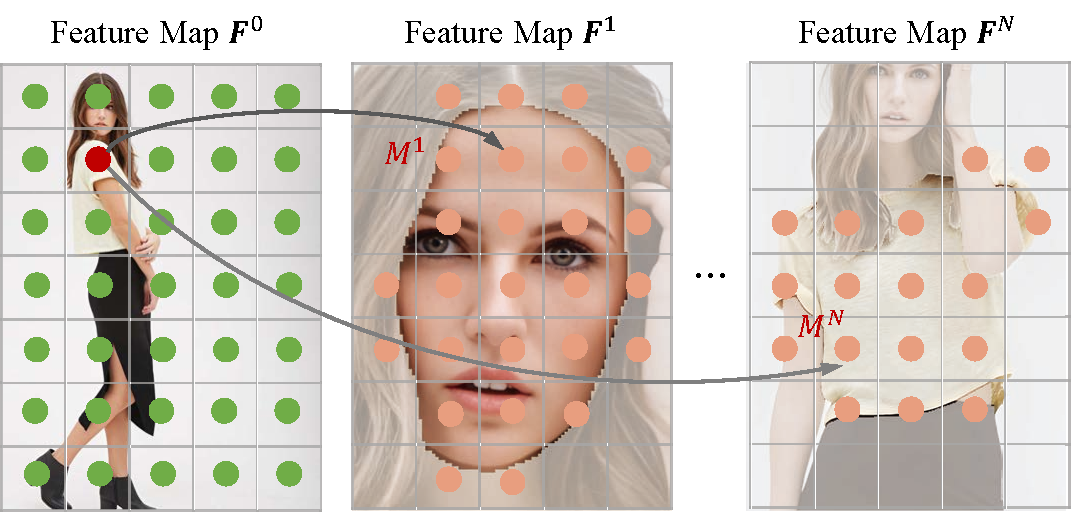
\includegraphics[width=\linewidth]{figure/mask_guided.pdf}
\caption{\textbf{Illustration of our Mask-Guided Attention.} For each patch $s$ (red point) on the feature map $\bm{F}^{0}$, given subject masks $M^{1:N}$ on the $N$ reference images, we only attend patch $s$ to features in these masks along with the patches on itself.}
\label{fig:mask_guided}
\end{figure}

\cparagraph{Semantic-Aware Appearance Encoder.} In image conditioned generation tasks, previous work~\cite{ye2023ipadapter,yang2023paintbyexample,zhang2024ssrencoder} employs CLIP image encoder~\cite{radford2021clip}, or combined with some simple linear layers to encode reference images, thereby replacing the original text encoder in Stable Diffusion~\cite{rombach2022ldm}. However, such methods struggle to preserve appearance details due to the loss of spatial representations when encoding the reference images into semantic-level features.

Inspired by recent works~\cite{referenceonlycontrol,cao2023masactrl,xu2023magicanimate,hu2023animateanyone} on dense reference image conditioning, we propose a semantic-aware appearance encoder with improved identity and details preservation. Specifically, we adopt a framework identical to the denoising U-Net for the appearance encoder. Unlike the denoising branch, we do not add any noise to the reference images. Given $N$ images capturing various parts of human appearance, we first compress them into latent features and then input them into the copied trainable U-Net. Instead of simply piecing multiple reference images together, we pass the latent features of different parts through the appearance encoder one by one and provide a textual class label for each part. These text labels, such as face, hair, upper body clothes, etc., are converted into feature representations by CLIP text encoder~\cite{radford2021clip} and then injected into the appearance encoder through cross-attention. This simple yet effective external condition provides a classifier-like guidance, which enables the encoder to have semantic awareness of different parts of the human appearance rather than simply performing operations such as image downsampling and upsampling. This helps produce results that are not only rich in detail, but also flexible and realistic.

In the encoding process, we set the timestep to 0 and only perform one processing instead of iterating successively, so it will not cause time burden at the inference stage. We cache the features before each self-attention layer for the next multi-image conditioned generation.

\cparagraph{Shared Self-Attention.} After obtaining the multi-layer feature maps of $N$ reference images, we do not directly add them to the features in denoising U-Net, but use shared keys and values in self-attention to achieve feature injection. This is because our reference and target images are not structurally aligned.

Take one certain self-attention layer as an example. Given the features of $N$ reference images $\bm{F}^{1:N}$ and the feature maps $\bm{F}^{0}$ in the denoising U-Net, we concatenate the feature maps of them side-by-side as input to the self-attention layer, denoted as $[\bm{F}^{0}|\bm{F}^{1}|\cdots|\bm{F}^{N}]$. This allows each location $s$ on $\bm{F}^{0}$ to attend to all locations on itself and reference feature maps, calculated as:
\begin{equation}
\begin{split}
    \tilde{\bm{F}}_{s}^{0} =&\ \text{SoftMax}\left(
    \frac{
    Q(\bm{F}_s^0)\cdot K([\bm{F}^{0}|\bm{F}^{1}|\cdots|\bm{F}^{N}])^{\top}
    }{
    \sqrt{d}
    }\right)  \\
    & \cdot V([\bm{F}^{0}|\bm{F}^{1}|\cdots|\bm{F}^{N}])
    \label{eq:vanilla_self_attn}
\end{split}
\end{equation}

We retain the cross-attention layers in Stable Diffusion~\cite{rombach2022ldm} for injecting CLIP features of reference images and optional text input. We use the decoupled cross-attention proposed by IP-Adapter~\cite{ye2023ipadapter} to support both images and text input. Specifically, feature maps $\tilde{\bm{F}}^{0}$ obtained from shared self-attention serve as the origin of the query, and the reference image features and text features are each used as the key and value of the two cross-attention. The final feature maps are the sum of the two cross-attention outputs.

To further enhance the controllability of the human image generation, we add the pose map as an additional control. We construct a tiny convolution network, which is similar to the condition embedding network in ControlNet~\cite{zhang2023controlnet}, to extract the features of the pose map. The features are then added to the initial feature maps in the denoising U-Net.

\cparagraph{Enhanced Mask-Guided Subject Selection.}
We find that the vanilla shared self-attention leads to interference from irrelevant subjects in the reference images (shown in the 6th column in Fig.~\ref{fig:ablation}), resulting in an unnatural appearance and background. To synthesize human images conditioned on specified parts from each reference image, we enhance the vanilla self-attention mechanism by incorporating subject masks in the reference images. Fig.~\ref{fig:mask_guided} presents this mechanism. Starting with a patch $s$ on a feature map $\bm{F}^{0}$ in the denoising U-Net, and subject masks $M^{1:N}$ on the $N$ reference images. When computing the attention map between the one in the denoising U-Net and those from the appearance encoder, patches that do not lie in these masks are ignored. Hence, the target patch $s$ only has access to features of the subjects specified by masks in the reference images, thereby avoiding interference from other elements such as the background. The final formulation of the mask-guided attention is defined as follows:
\begin{equation}
\begin{split}
    \tilde{\bm{F}}_{s}^{0} =&\ \text{SoftMax}\left(
    \frac{
    Q(\bm{F}_s^0)\cdot K([\bm{F}^{0}|\cdots|\bm{F}^{N}_{M^{N}}])^{\top}
    }{
    \sqrt{d}
    }\right)\\
    & \cdot V([\bm{F}^{0}|\cdots|\bm{F}^{N}_{M^{N}}])
    \label{eq:mask_guided_self_attn}
\end{split}
\end{equation}

In practice, to avoid misalignment between masks and original images caused by downsampling, a full-ones convolutional kernel is applied to the mask before each attention layer, ensuring that the mask preserves critical regions. Overall, the mask-guided attention enhances the ability of Parts2Whole to precisely extract the appearance of specified subjects in reference images.
